\section{Stand der Forschung} 


\subsection*{Continuous Humanoid Locomotion over Uneven Terrain using Stereo Fusion}

    \begin{frame}[t]
    \frametitle{Stand der Forschung: Continuous Humanoid Locomotion over Uneven Terrain using Stereo Fusion}

    \begin{columns}[t]
      \column[]{6cm}
      
      \begin{itemize}
      \item Team MIT's Ansatz für Fortbewegung auf unebenem Gelände anlässlich DRC Finale
      \item Basiert auf Kintinous
      \begin{itemize}
       \item 3D-TSDF-Struktur für RGB-D Sensorfusion
       \item CUDA-Beschleunigung für Echtzeit-Anwendung
%        \item Verschiebendes Voxelgitter auf GPU ermöglicht größere Szenen 
      \end{itemize}

      \item Anpassung von Kintinous für Stereo Kamera (ATLAS Roboter)
%       \item 3D-Karte genutzt für Fußschrittplanung und Kollisionsvermeidung

     \end{itemize}
     

      \column{6cm}
      
       \begin{figure}[h]
 	\centering
%  	    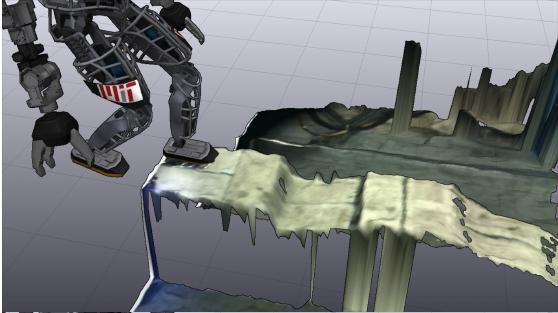
\includegraphics[width=\textwidth]{images/mit_locomotion}
	  \movie[width = 6cm, height = 3.5cm,
                 autostart,loop, poster] 
      {}{video/mit.m4v}
 	\caption{Laufen basierend auf Kintinous [2]} 
       \end{figure}
  
    \end{columns}
    \end{frame}

    
    \begin{frame}[t]
    \frametitle{Stand der Forschung: Continuous Humanoid Locomotion over Uneven Terrain using Stereo Fusion}

    \begin{columns}[t]
      \column[]{6cm}
      \vspace{-0.5cm}
      \begin{exampleblock}{Vorteile}
	  \begin{itemize}
	    \item Performant durch GPU-Beschleunigung
	  \end{itemize} 
	\end{exampleblock}
	
	\begin{alertblock}{Nachteile}
	 \begin{itemize}
	\item GPU-Nutzung schränkt mögliche Anwendungsfälle ein
	\item Gebiete außerhalb des Kamera-Blickfeldes werden tesseliert 
	\begin{itemize}
	\item Löschen der TSDF-Daten
	\end{itemize}
	\item Unterstützung von nur einem Sensor

      \end{itemize}
	\end{alertblock}
     

      \column{6cm}
      
       \begin{figure}[h]
 	\centering
%  	    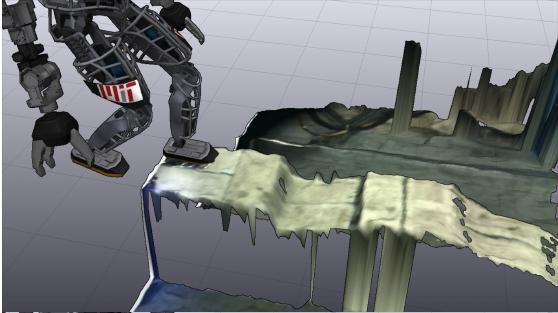
\includegraphics[width=\textwidth]{images/mit_locomotion}
	  \movie[width = 6cm, height = 3.5cm,
                 autostart,loop, poster] 
      {}{video/mit.m4v}
 	\caption{Laufen basierend auf Kintinous [2]} 
       \end{figure}
  
    \end{columns}
    \end{frame}

 \subsection*{Robot-Centric Elevation Mapping}
 
    \begin{frame}[t]
    \frametitle{Stand der Forschung: Robot-Centric Elevation Mapping}

    \begin{columns}[t]
      \column[]{6cm}
      
      \begin{itemize}
      \item  ETH Zürich, 2014
      \item  Erstellung von Höhenkarten (2,5D) für mobile Roboter 
      \item  Kalman-Filter für Fusion der Höhenschätzungen inklusive Abschätzung von Unsicherheit
      \item  ROS-Integration 
      \item  CPU-basiert


     \end{itemize}
     

      \column{6cm}
      
       \begin{figure}[h]
 	\centering
%  	    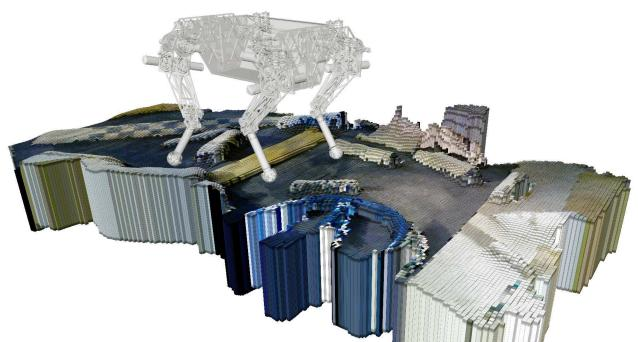
\includegraphics[width=\textwidth]{images/eth_elevation_mapping}
 	  \movie[width = 6cm, height = 3.4cm,
                 autostart,loop, poster] 
{}{video/eth.mp4}
 	\caption{Erstellung der Höhenkarte [3]} 
       \end{figure}
  
    \end{columns}
    \end{frame}

    \begin{frame}[t]
    \frametitle{Stand der Forschung: Robot-Centric Elevation Mapping}
      
      \begin{columns}[t]
      \column[]{6cm}
      \vspace{-0.5cm}
        
	\begin{exampleblock}{Vorteile}
	  \begin{itemize}
	    \item Anwendung auf vielen Robotersystemen möglich durch CPU-Nutzung
	    \item 2,5D Darstellung
	    \begin{itemize}
	    \item Hohe Aktualisierungsrate
	    \item Geringer Speicherverbrauch
	    \end{itemize} 

	  \end{itemize} 
	\end{exampleblock}
	
	\begin{alertblock}{Nachteile}
	\begin{itemize}
	  \item Nur ein Distanzsensor unterstützt
	  \item Form der Weltdarstellung nicht immer geeignet
	\end{itemize}

	\end{alertblock}
     
     \column{6cm}
      
       \begin{figure}[h]
 	\centering
 	    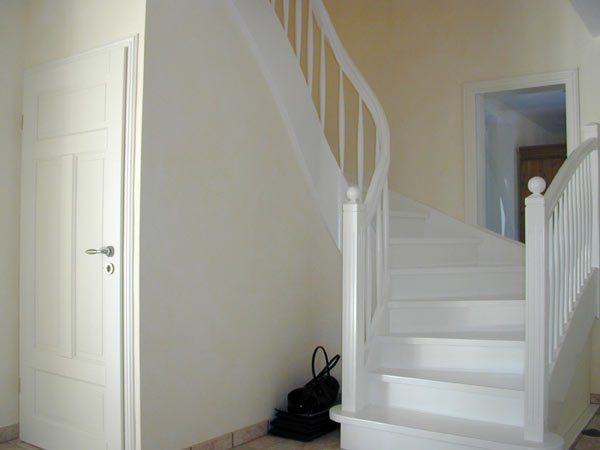
\includegraphics[width=\textwidth]{images/raum_unter_treppe}
 	\caption{Raum unter Treppe   [4]} 
       \end{figure}
  
    \end{columns}
     
    \end{frame}
    
    
    
\subsection*{Obviously}


    \begin{frame}[t]
    \frametitle{Stand der Forschung: Obviously}
      
      \begin{columns}[t]
      \column[]{7cm}
      
      \begin{itemize}
      \item TH Nürnberg, 2014
      \item Multisensor-Fusions-Framework für Umgebungsmodellierung
      \item Echtzeit-Anwendung für mobile Roboter
      \item CPU-gestütztes TSDF
     % \item Hinzufügen von neuen Sensoren: Implementierung des Sensormodell-Interfaces
      \item Keine ROS-Integration 
      
      
     \end{itemize}
     
     \column{5cm}
      
       \begin{figure}[h]
       \vspace{-0.5cm}
 	\centering
 	    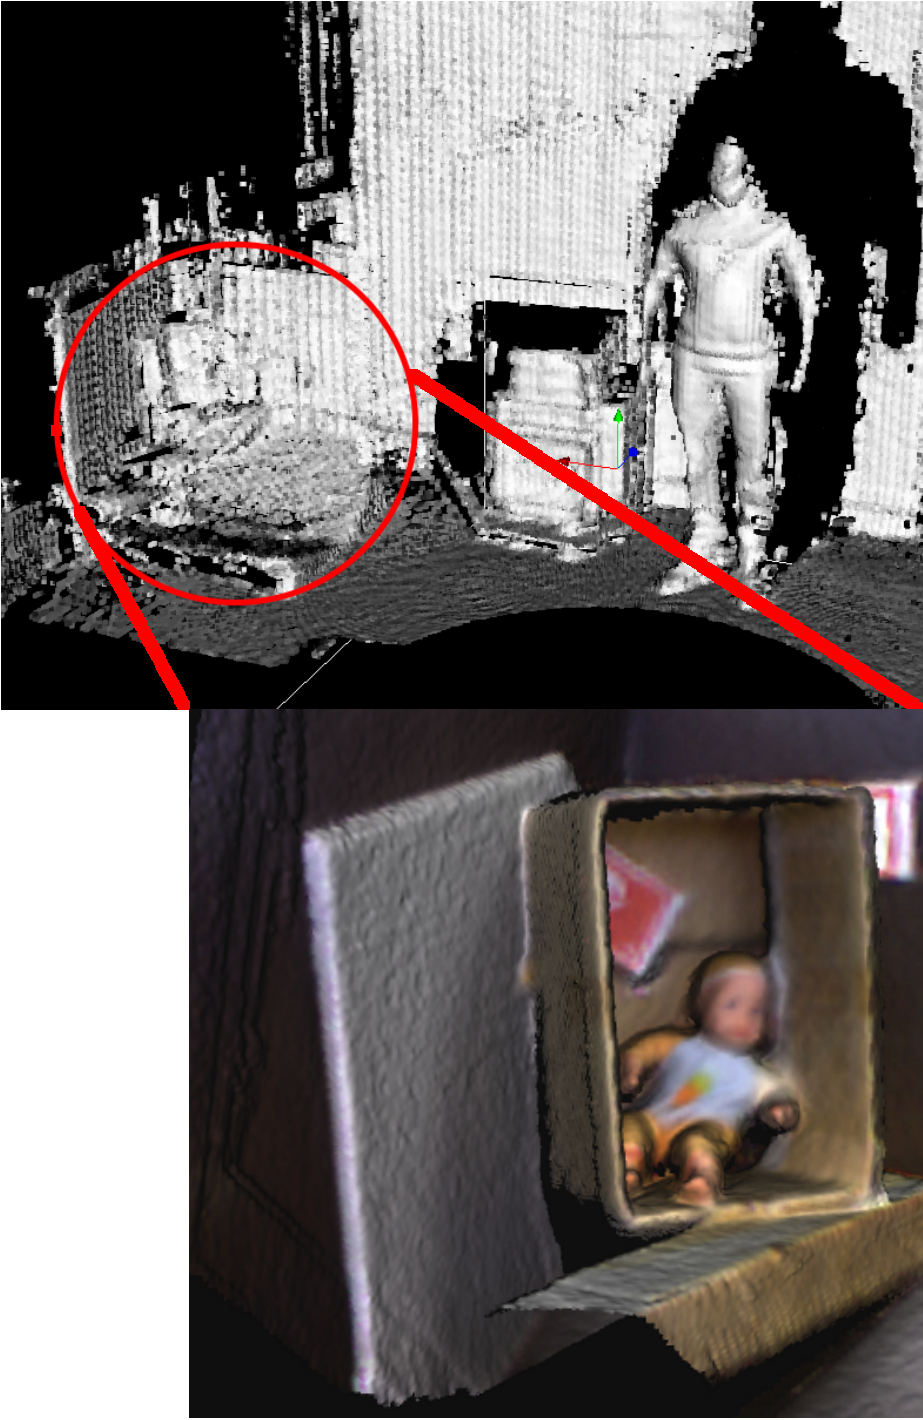
\includegraphics[width=0.65\textwidth]{images/obviosly_concat}
 	\caption{Einsatz von Obviously [5]} 
       \end{figure}
  
    \end{columns}
     
    \end{frame}
    
    \begin{frame}[t]
    \frametitle{Stand der Forschung: Obviously}
      
      \begin{columns}[t]
      \column[]{7cm}
      \vspace{-0.5cm}
        \begin{exampleblock}{Vorteile}
	  \begin{itemize}
	    \item Mehrere Sensoren fusionierbar
	    \item Verschiedene Repräsentationen für Weltmodell verfügbar
	  \end{itemize} 
	\end{exampleblock}
	
	\begin{alertblock}{Nachteile}
	        \begin{itemize}
	\item Voxelgitter für TSDF-Daten
	\item Leere Voxelblöcke werden gespeichert und aktualisiert\\
	$\rightarrow$ Unnötige Verwendung von Speicher und Rechenzeit 
	\item Hinzufügen von neuen Sensoren aufwendig 
      \end{itemize} 
	\end{alertblock}
     
     \column{5cm}
      
       \begin{figure}[h]
       \vspace{-0.5cm}
 	\centering
 	    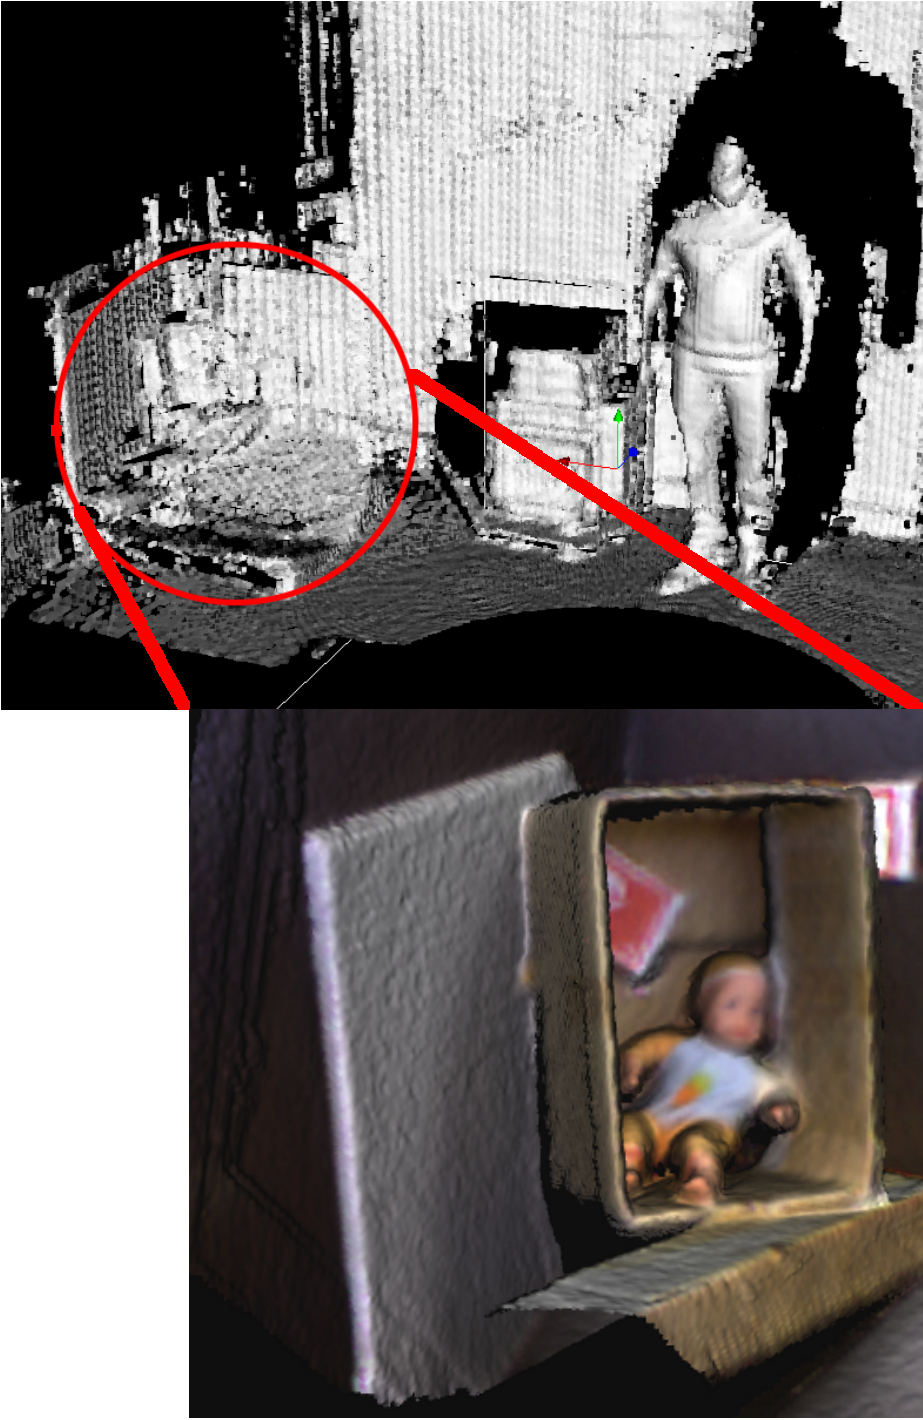
\includegraphics[width=0.65\textwidth]{images/obviosly_concat}
 	\caption{Einsatz von Obviously [5]} 
       \end{figure}
  
    \end{columns}
     
    \end{frame}
    
\subsection*{Vigir Terrain Classifier}

\begin{frame}[t]
  \frametitle{Stand der Forschung: Vigir Terrain Classifier}
      
     \begin{columns}[t]
      \column[]{6cm}
     
      \begin{itemize}
	\item Akkumulation von Laserscans
	\item Octree mit fester Knotengröße
	\item Erzeugt Höhenkarte und Oberflächennormalen-Schätzung
	\item Nur Daten im Bereich um neusten Laserscan geupdated
      \end{itemize} 
     
     \column{6cm}
     

       \begin{figure}[h]
       \vspace{-0.5cm}
	  \movie[width = 6cm, height = 3.5cm,
                 autostart,loop, poster] 
{}{video/drop.avi}
 	\caption{Laufen mit Vigir Terrain Classifier [6]} 
       \end{figure}

  
    \end{columns}  
      
\end{frame}


\begin{frame}[t]
  \frametitle{Stand der Forschung: Vigir Terrain Classifier}
      
     \begin{columns}[t]
      \column[]{6cm}
      
       \begin{exampleblock}{Vorteile}
	  \begin{itemize}
	  %\item Nur eine Datenschicht
	    \item Hohe Aktualisierungsraten möglich
	  \end{itemize} 
	\end{exampleblock}
	  
	\begin{alertblock}{Nachteile}
	  \begin{itemize}
	      %\item Nur eine Datenschicht
		\item Keine Abschätzung der Sicherheit von Höhenmessungen
		\item Dynamische Objekte "`zerstören"' Umgebungsmodellierung
		\item Nur ein Sensor wird unterstützt
	      \end{itemize} 
	    \end{alertblock}
	    
     \column{6cm}

       \begin{figure}[h]
       \vspace{-0.5cm}
	  \movie[width = 6cm, height = 3.5cm,
                 autostart,loop, poster] 
{}{video/vigir_terrain.mp4}
 	\caption{Laufen mit Vigir Terrain Classifier [6]} 
       \end{figure}

  
    \end{columns}  
      
\end{frame}

 \subsection*{CHISEL}
 
\begin{frame}[t]
  \frametitle{Stand der Forschung: CHISEL}
  
  \begin{columns}[t]
      \column[]{6cm}
      
      \begin{itemize}
      \item CMU, 2015
      \item Bibliothek für 3D-Rekonstruktion großer Volumen in Echtzeit
      \item Ursprünglich für mobile Geräte mit Tiefensensor
      \item Spatially-hashed TSDF nur mit CPU
     % \begin{itemize}
       %\item Experiment: 93\% der Voxel leer
       %\item Wieso speichern und aktualisieren?
      %\end{itemize}

      \item Beachtung von Sensor-Messfehlern
     \end{itemize}
     
     \column{6cm}
      
      \begin{figure}[h]
%  	\centering
% 	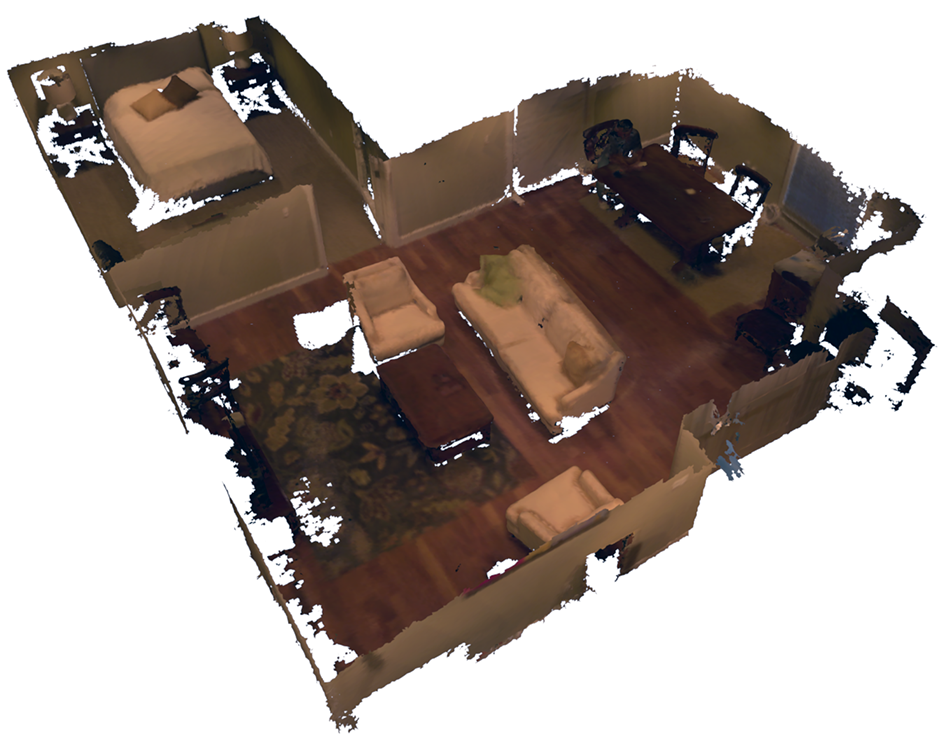
\includegraphics[width=0.65\textwidth]{images/chisel}
	  \movie[width = 6cm, height = 3.5cm,
                 autostart,loop, poster] 
{}{video/chisel_trim.m4v}
 	\caption{Szene rekonstruiert durch CHISEL [7]} 
      \end{figure}
  
    \end{columns}
\end{frame}

\begin{frame}[t]
  \frametitle{Stand der Forschung: CHISEL}
  
  \begin{columns}[t]
      \column[]{6cm}
      
  \begin{exampleblock}{Vorteile}
  \begin{itemize}
    \item ROS-Integration
    \item Sehr leistungsfähige Bibliothek
    \item TSDF-Daten bleiben erhalten
  \end{itemize} 
  \end{exampleblock}
  
  \begin{alertblock}{Nachteile}
    \begin{itemize}
      \item Support für nur einen Distanzsensor
      \item Keine Posenschätzung vorhanden \\ $\rightarrow$ externe Posenschätzung benötigt
    \end{itemize} 
  \end{alertblock}
     
     \column{6cm}
      
      \begin{figure}[h]
%  	\centering
% 	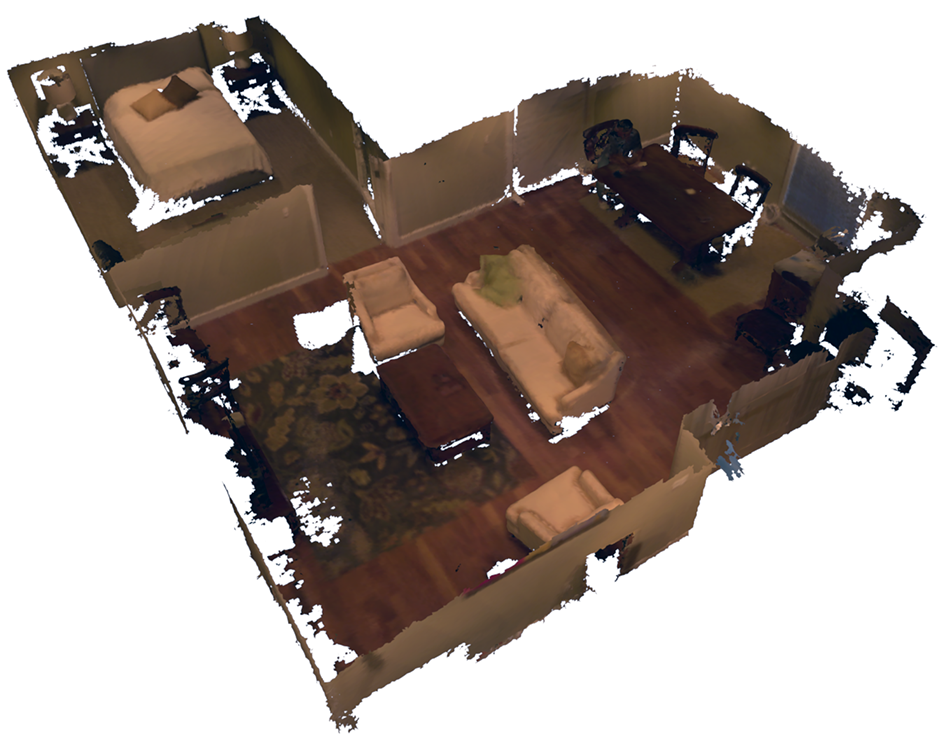
\includegraphics[width=0.65\textwidth]{images/chisel}
\movie[start=35s,width = 5.5cm, height = 3.5cm,
                 autostart,repeat,poster] 
{}{video/chisel_trim.m4v}
 	\caption{Szene rekonstruiert durch CHISEL [7]} 
      \end{figure}
  
    \end{columns}
\end{frame}

